\documentclass[12pt,a4paper]{article}
\title{Perceptron}
\author{Hanxiao Du}
\date{}

\usepackage{amsmath}
\usepackage{amssymb}
\usepackage{amsthm}
\usepackage{bbm}
\usepackage{pifont}
\usepackage{marvosym}
\usepackage{mathtools}
\usepackage{environ}
\usepackage{lipsum}
\usepackage{undertilde}
\usepackage{hyperref}
\usepackage{graphicx}
\hypersetup{colorlinks=true,
     linkcolor=black,urlcolor=blue}

\usepackage[total={6in, 10in}]{geometry}
\newtheorem{theorem}{Theorem}
\setlength{\parindent}{0pt}
\renewcommand{\qedsymbol}{$\blacksquare$}
\DeclareMathOperator*{\argmax}{\arg\!\max}
\DeclareMathOperator*{\argmin}{\arg\!\min}

\begin{document}
\maketitle
\tableofcontents

\section{Linear Classifiers}

For now, we only consider thresholded linear mappings from inputs to
(binary) outputs (for binary classification):

\begin{align}
f(x;\theta)=sign(\theta_1x_1+\cdots+\theta_dx_d)=sign(\theta^Tx)
\end{align}

where \(x=[x_1,\cdots,x_d]^T\) is a matrix (column vector) of the input
(i.e.~input with \(d\) attributes, \(x_i\) for all \(i \in [d]\) denotes
an attribute of the input), \(\theta = [\theta_1,\cdots,\theta_d]^T\) is
matrix (column vector) of the parameters (or coefficients, \(\theta_j\)
for all \(j \in [d]\) denotes the coefficient of the \(j\)-th
attribute), also

\begin{equation}
sign(x)=\begin{cases} 1 \text{ if } x\geq0,\\ -1 \text{ if } x <0 \text{.}\end{cases}
\end{equation}

\begin{figure}[h]
\centering
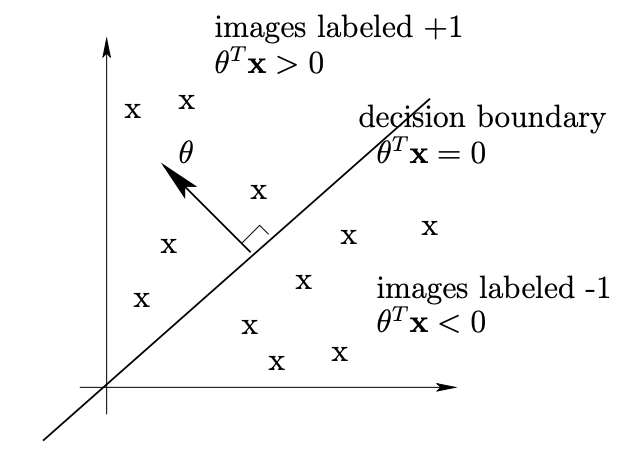
\includegraphics[scale=0.7]{assets/figures/linear_classifier.png}
\caption{A linear classifier through origin.\label{linear_cls}}
\end{figure}

\begin{itemize}
\item
  The functions in the class are parameterized by \(\theta\).
\item
  \(f(x;\theta)\) defines a plane in \(d\)-dimensions.
\item
  The decision boundary is \(\theta^Tx=0.\) Thus, the parameter vector
  \(\theta\) is orthogonal to the decision boundary.
\item
  The decision boundary goes through the origin since \(x=0\) satisfies
  \(\theta^Tx=0.\)
\end{itemize}



\section{Perceptron}

After choosing a class of functions, we still have to find a specific
function in this class that performs well on the training set. This is
usually referred to as the estimation problem.

We would like to find a linear classifier that makes the fewest mistakes
on the training set, i.e.~find \(\theta\) that minimizes the training
error:

\begin{align} \hat{E}[\theta]=\frac{1}{n} \displaystyle\sum_{i=1}^n \big[\mathbb{I}(y_i=f(x_i;\theta))\big]\\=\frac{1}{n}\displaystyle\sum_{i=1}^n \big[1-\delta(y_i, f(x_i;\theta))\big]\\=\frac{1}{n}\displaystyle\sum_{i=1}^n Loss(y_i, f(x_i;\theta))\text{,}\end{align}

where \(\delta(y, y^\prime) =1\) if \(y=y^\prime\) and 0 otherwise. The
training error merely counts the average occurrence of that the labels
\(y_i\) is different from the model predicted value
\(f(x_i; \theta)\ \forall i \in [n]\), which can also be expressed in
terms of a loss function \(Loss(y_i, f(x_i;\theta))\).

Loss function is useful when errors of a particular kind cost more than
other. For the case above, we are using zero-one loss for simplicity.

In this case, the simplest algorithm to minimize the training error is
the perceptron update rule.

\begin{equation}\theta^\prime \leftarrow \theta + y_ix_i \text{ if } y_i \neq f(x_i;\theta)\end{equation}

This update rule only changes \(\theta\) if the model predicted
incorrectly.

\begin{itemize}
\item
  the model made a mistake on \(x_i\):
  \(y_i \neq f(x_i;\theta) \iff y_i\theta^Tx_i <0\)
\end{itemize}

Suppose we make a mistake on \(x_i\) (i.e.~\(y_i\theta^Tx_i <0\)), then
after the update \(\theta^\prime \leftarrow \theta + y_ix_i\), consider
classifying the same image \(x_i\):

Thus, \(y_i\theta^Tx_i\) increased after the update (i.e.~it becomes
more positive/correct).

\begin{align}y_i\theta^{\prime^T}x_i=y_i(\theta+y_ix_i)^Tx_i \\=y_i\theta^Tx_i+y_i^2x_i^Tx_i\\=y_i\theta^Tx_i+y_i^2||x_i||_2^2\end{align}

\subsection{Analysis of The Perceptron
Algorithm}

The perceptron algorithm stops to update the parameters only when all
the training images are classified correctly. Thus, if it is possible to
classify all training data with a linear classifier, the perceptron
algorithm will find such a classifier eventually in a finite number of
updates.

\end{document}
